
\documentclass[twoside]{article}
\usepackage{CJKutf8}

%\usepackage{graphics}
\usepackage{graphics}
\usepackage{geometry}
\usepackage{forest,amsmath}
\usepackage{enumerate}
\usepackage{url}
\usepackage{latexsym,bm,amssymb}

\geometry{left=2.5cm,right=2cm,top=2.5cm,bottom=2.5cm}

%\setlength{\oddsidemargin}{0.25 in}
%\setlength{\evensidemargin}{-0.25 in}
%\setlength{\topmargin}{-0.6 in}
%\setlength{\textwidth}{6.5 in}
%\setlength{\textheight}{8.5 in}
%\setlength{\headsep}{0.75 in}
\setlength{\parindent}{0 in}
\setlength{\parskip}{0.1 in}

\usepackage{listings}
\usepackage{color}
\renewcommand\lstlistingname{Quelltext} % Change language of section name
\lstset{ % General setup for the package
    language= C,
    %basicstyle=\small\sffamily,
    basicstyle=\ttfamily,
    numbers=left,
     numberstyle=\tiny,
    frame=tb,
    tabsize=4,
    columns=fixed,
    showstringspaces=false,
    showtabs=false,
    keepspaces,
    commentstyle=\color{red},
    keywordstyle=\color{blue}
}

%
% The following commands set up the lecnum (lecture number)
% counter and make various numbering schemes work relative
% to the lecture number.
%
%\newcounter{lecnum}
%\renewcommand{\thepage}{\thelecnum-\arabic{page}}
%\renewcommand{\thesection}{\thelecnum.\arabic{section}}
%\renewcommand{\theequation}{\thelecnum.\arabic{equation}}
%\renewcommand{\thefigure}{\thelecnum.\arabic{figure}}
%\renewcommand{\thetable}{\thelecnum.\arabic{table}}

%
% The following macro is used to generate the header.
%


%


%Use this command for a figure; it puts a figure in wherever you want it.
%usage: 
%\begin{figure}
%\begin{center}
%\includegraphics[width=5in]{fig-file}
%\caption{}\label{fig:delavl}
%\end{center}
%\end{figure}

%%% Use the following command for a table
%%%

% Use these for theorems, lemmas, proofs, etc.
\newtheorem{theorem}{Theorem}[theorem]
\newtheorem{lemma}[theorem]{Lemma}
\newtheorem{proposition}[theorem]{Proposition}
\newtheorem{claim}[theorem]{Claim}
\newtheorem{corollary}[theorem]{Corollary}
\newtheorem{definition}[theorem]{Definition}
\newenvironment{proof}{{\bf Proof:}}{\hfill\rule{2mm}{2mm}}

% **** IF YOU WANT TO DEFINE ADDITIONAL MACROS FOR YOURSELF, PUT THEM HERE:

\begin{document}
\begin{CJK*}{UTF8}{gbsn}
	%FILL IN THE RIGHT INFO.
	%\lecture{**LECTURE-NUMBER**}{**DATE**}{**LECTURER**}{**SCRIBE**}
	%\lecture{1}{Project Name}{Deshi Ye}{Student 1, Student 2, 学生3}
	%\footnotetext{These notes are partially based on those of Nigel Mansell.}
	\title{Hexadecimal}
	\date{}
	%\maketitle
	% **** YOUR NOTES GO HERE:

	% Some general latex examples and examples making use of the
	% macros follow.  
	%**** IN GENERAL, BE BRIEF. LONG SCRIBE NOTES, NO MATTER HOW WELL WRITTEN,
	%**** ARE NEVER READ BY ANYBODY.
	\section{Introduction}

	In this program, we are required to write a program with LC-3 assembly language, which can convert the decimal numbers to hexadecimal one.For example, 
	
	if the user input$$123$$
	
	The program should print  $$007B$$
	

	\section{Algorithm Specification}
	Initially, we devide the program into four functional block:
	\begin{itemize}
		\item store the input characters
		\item convert ASCII characters into decimal digit
		\item convert the decimal digit into hexadecimal digit
		\item convert hexadecimal digit into ASCII characters and output
	\end{itemize}
	
	Firsty, in the input part, use \textbf{TRAP x20 and TRAP x21} to read the input character, compare it with CR, if it's not CR, then continue to read. Also the program will record the number of characters inputted.
	
	Next, in the ASCII-to-decimal-digit conversion, we use $result:= 10result + number$	to calculate the decimal digit
	
	Then, the program converts the dicimal digit to hexadecimal digit by dividing it with 16 four times. Each time, we store the remainder as the result hexadecimal digit, and assign the quotien as the dicimal digit in the next loop. In the dividing procedure, the sign of the digit should be paid attention to. So in the program, we divide it into two cases. After the decimal digit been transfered into hexadecimal digit, we store the result into memory.
	
	Finally, we check each four hexadecimal digit wheteher they are less than 10, then transfer it into corresponding ASCII characters and use \textbf{TRAP x21} to output them.

	The peseudocode is follow:
	\begin{lstlisting}[mathescape=true]
		n $\leftarrow$ 0
		while(input != \n)
			c[n++] = input // array storing characters
		result $\leftarrow$ 0 
		for i = 0 to n - 1
			result $\leftarrow$ result<<3 + result<<1 + c[i] - x0030
		if(result>32767) // the first bit is 1
			result $\leftarrow$ result - 32768
			quotient $\leftarrow$ result/16 + 1
			result $\leftarrow$ result - quotien*16 + x7fff + x0001
			quotient $\leftarrow$ quotient + result/16
			hex[3] $\leftarrow$ result - quotient * 16 
			result $\leftarrow$ quotient
			for i = 1 to 3
				quotient $\leftarrow$ result/16
				hex[3-i] $\leftarrow$ result - quotient*16
				result $\leftarrow$ quotient
				
		else 			//the first bit is 0
			for i = 1 to 4
				quotient $\leftarrow$ result/16
				hex[4-i] $\leftarrow$ result - quotient*16
				result $\leftarrow$ quotient
		for i = 1 to 4
			if hex[i-1]<10
				output $\leftarrow$ hex[i-1] + x0030
			else 
				output $\leftarrow$ hex[i-1] + x0041
		

	\end{lstlisting}

	In the peseudocode, the / operator is implement as follow:
	
	\begin{lstlisting}[mathescape=true]
		quotient $\leftarrow$ 0
		remainder $\leftarrow$ 0
		while  dividend > 0
			dividend $\leftarrow$ dividend - 16
			quotient++
		remainder $\leftarrow$ dividend + 16
	\end{lstlisting}

	\section{Q and A}
	\begin{itemize}
		\item 	Q: what the procedure of your input and output block?
		
				A: In the input procedure, we use trap x20 and trap x21 to read the character and echo it. Then we store the character into memory.
				
				In the output procedure, we use the hexadecimal digit calculated before, transfer it into ascii character and use trap x21 to output it.
		\item	Q: Is your program use divide operation?
		
				A: yes. In the program, divide operation is used to transform the decimal digit into hexadecimal digit.
	\end{itemize}


	\section{essential parts of code}
	Fig 1 is the code to transfer the ascii character to digit
	\begin{figure}[htbp]
		\small
		\centering
		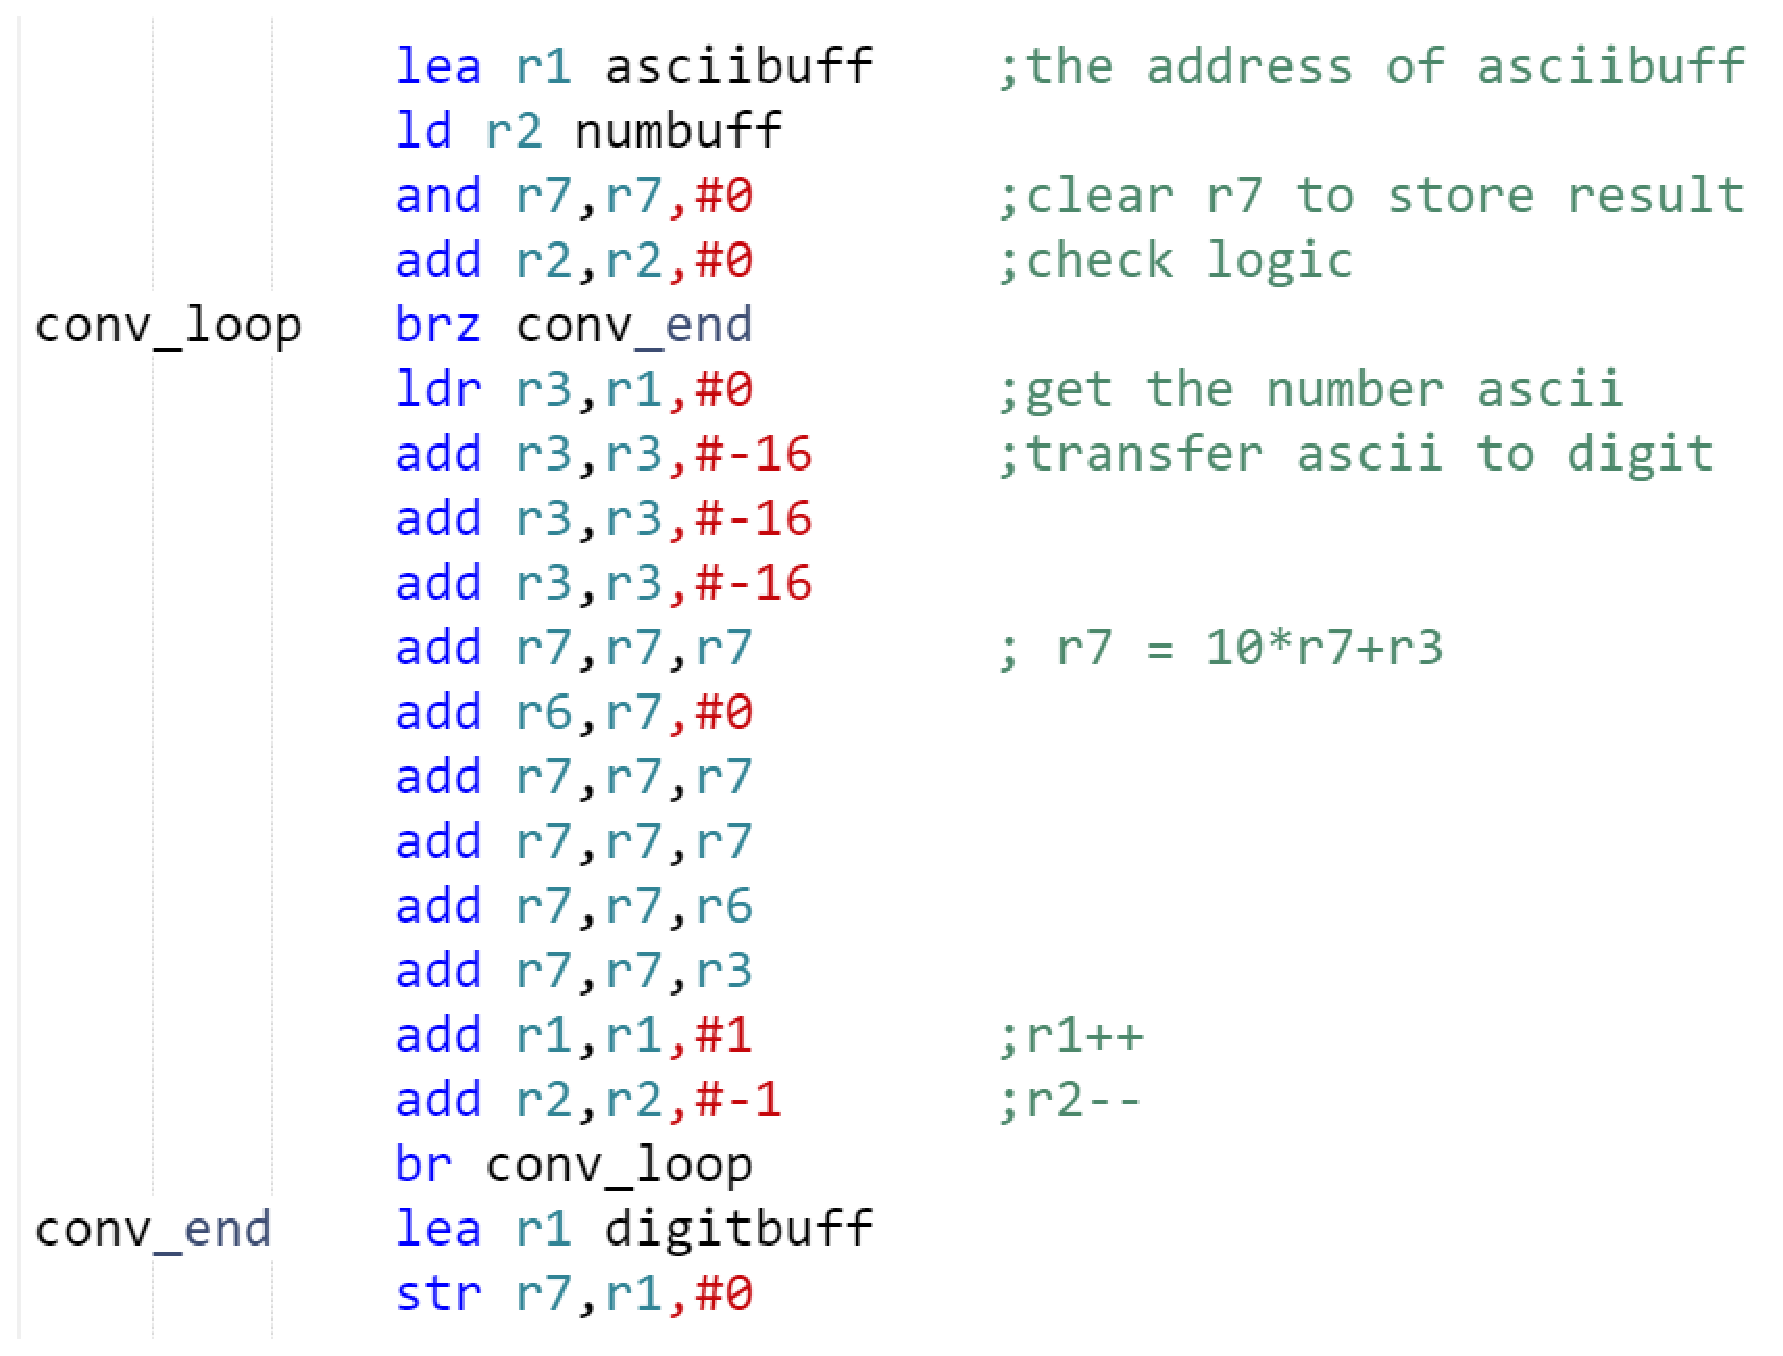
\includegraphics[width=0.7\textwidth]{fig1.eps}
		\caption{Fig 1} %名字
	\end{figure}
	
	
	Fig 2 is transfer the decimal digit to hexadecimal digit code(positive case)

	\begin{figure}[htbp]
		\small
		\centering
		\includegraphics[width=0.7\textwidth]{fig2.eps}
		\caption{Fig 2} %名字
	\end{figure}

\end{CJK*}
\end{document}





